\section{Dijagram toka podataka (DFD)}

Dijagram toka podataka prikazuje kako se podaci kreću kroz informacioni sistem. Uključuju odakle podaci dolaze, koji procesi ih obrađuju, gde se čuvaju i kome se vraćaju. Fokusira se na podatke koji se razmenjuju, a ne prikazuju redosled koraka u kojima se koriste. U nastavku su prikazana dva dijagrama, kontekstni koji prikazuje ceo informacioni sistem kao jedan proces i dijagram toka podataka (nivo 0) koji razlaže sistem na procese koji odgovaraju slučajevima upotrebe.

\begin{figure}[H]
	\centering
	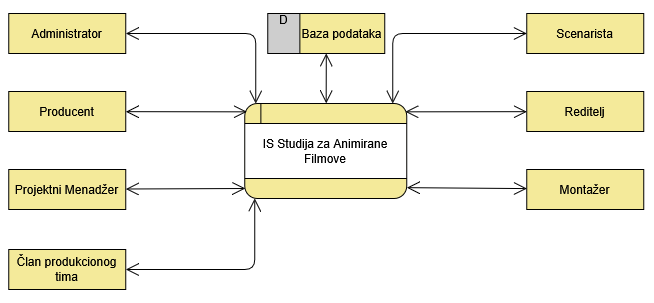
\includegraphics[width=\textwidth]{./dijagrami/dijagram_konteksta/dijagram_konteksta.png} 
	\caption{Dijagram konteksta}
\end{figure}

\begin{figure}[H]
	\centering
	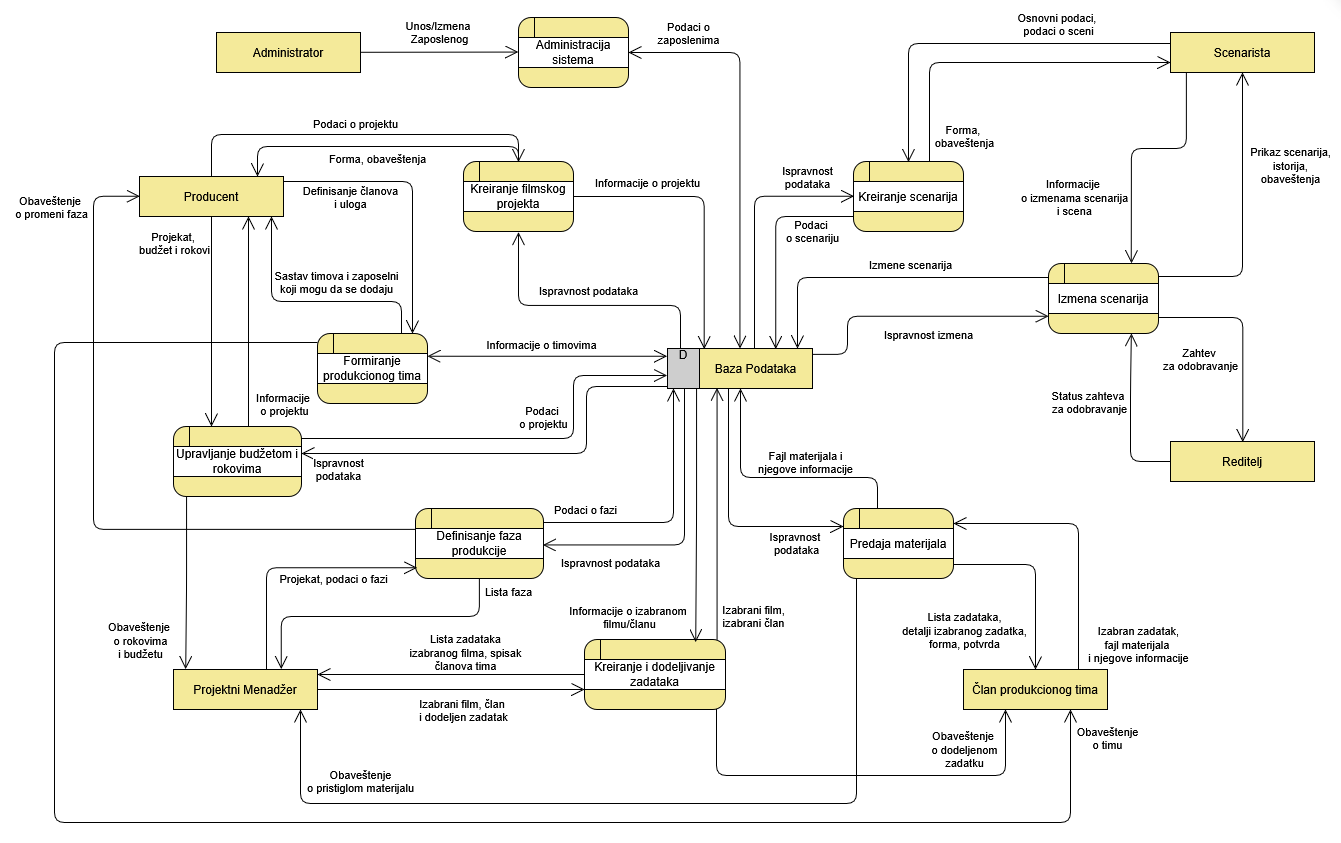
\includegraphics[width=\textwidth]{./dijagrami/dfd/dijagram_toka_podataka_nivo0.png} 
	\caption{Dijagram toka podataka - nivo 0}
\end{figure}
